\chapter{Oscillations}
\textcolor{red}{This chapter needs to have pictures added to it.}
\section{SHM and Sine Waves}

There are many places in everyday life where we encounter oscillations. Some examples include:
\begin{itemize}
\setlength{\itemsep}{-5pt}
    \item A car travelling over a speed bump and bounces up and down,
    \item A person on a swing,
    \item An object on a spring moving up and down,
    \item A small pendulum moving to and fro.
\end{itemize} 

An oscillating object moves first in one direction then in the other direction in what is called a cycle. This involves an object starting away from equilibrium and moving towards it, overshooting and then turning around.\\

In other words, during an oscillation the objects displacement from equilibrium changes during the motion. In one full cycle after being released from a non-equilibrium position, the objects displacement:
\begin{itemize}
\setlength{\itemsep}{-5pt}
    \item Decreases as it returns towards equilibrium,
    \item Reverses and increases as it moves past equilibrium and away from it in the other direction,
    \item Decreases as it returns back towards equilibrium,
    \item Increases as it moves away from equilibrium and back to the starting point.
\end{itemize} 

We call the maximum displacement from equilibrium the \textbf{amplitude} of the oscillation. When there is no friction the oscillation is called a \textbf{free vibration}. The time it takes for one cycle to be completed is called the \textbf{period of oscillation} and has the symbol $T$. This is equivalent to the period for circular motion from the last section. \\

Similarly, the frequency of oscillations is the number of cycles per second and is given by
\begin{equation*}
f=\frac{1}{T}.
\end{equation*}

Another important notion is that of the phase of an oscillation, and the phase difference between two oscillations. Imagine two children on adjacent identical swings and assume that the oscillations have the same period $T$. If one child reaches their maximum displacement a time $\Delta t$ later than the other child then we say that they are out of phase. The \textbf{phase difference} is the fraction of a cycle that the swings differ by $\frac{\Delta t}{T}$.\\

For example, if $T=2.4\text{s}$ and $\Delta t=0.6\text{s}$, then the second child will always be $0.6/2.4=1/4$, or a quarter of a cycle out phase. In radians this is $2\uppi\Delta t/T=\uppi/2$.

\paragraph{Example 7.1:}Consider an object suspended from the lower end of a vertical spring. The object is displaced downward from equilibrium. It takes $9.6\text{s}$ to undergo $20$ complete cycles.
\begin{itemize}
\setlength{\itemsep}{-5pt}
    \item[a)] What is the period of oscillation?
    \item[b)] What is the frequency of oscillation?
\end{itemize}  
a) $T=9.6/20=0.48\text{s}$.\\

b) $f=1/T=1/0.48=2.08\text{Hz}$.\\


\paragraph{Simple Harmonic Motion.} An oscillating object speeds up as it returns to equilibrium and slows down as it moves away. You can see this explicitly when you do the Hooke's law and simple pendulum experiments in the lab sessions. Assuming that friction is negligible, the amplitude of oscillation remains constant and an oscillating object will keep oscillating forever. The position, velocity, and acceleration of the oscillating object all follow ``similar'' curves as a function of time\footnote{This relationship between position, velocity, and acceleration is essentially the definition of simple harmonic motion and you could have oscillating motion where they are not related in precisely this way.} as can be seen in \cref{fig: shm profile}.

\begin{figure}[ht]
    \centering
    \ThisAltText{ Plots of the displacement, velocity, and acceleration of an oscillating object showing that they follow trigonometric curves with different phases.}
   % \pdftooltip{
    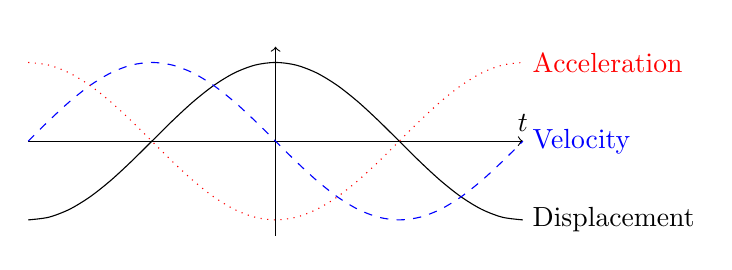
\begin{tikzpicture}[domain=-3.141:3.141, smooth,variable=\x]
     \draw[->] (-3.141,0) -- (3.141,0) node[above] {$t$};
  \draw[->] (0,-1.2) -- (0,1.2) node[above] {};
 \draw[color=black]   plot (\x,{cos(\x r)}) node[right] {Displacement};
  \draw[color=blue, dashed]   plot (\x,{-sin(\x r)}) node[right] {Velocity};
   \draw[color=red, dotted]   plot (\x,{-cos(\x r)})node[right] {Acceleration};
    \end{tikzpicture}
   % }{Displacement, velocity, and acceleration}
    \caption{Displacement, velocity, and acceleration of an oscillating object.}
        \label{fig: shm profile}
\end{figure}

By inspection of the plots in \cref{fig: shm profile} we see that the acceleration is always in the opposite direction to the displacement. This is because the velocity is the derivative (gradient) of displacement and acceleration is the gradient of velocity. Sometimes the force $F=ma$ is called a \textbf{restoring force} as it always points towards equilibrium and is trying to ``restore'' the object to its equilibrium position.\\

\textbf{Simple harmonic motion} (shm) is defined as oscillating motion where:
\begin{itemize}
\setlength{\itemsep}{-5pt}
    \item The acceleration is proportional to the displacement,
    \item and opposite in direction, ie $\vec{a}\propto -\vec{x}$.
\end{itemize} 
In other words, acceleration =-constant $\times$ displacement. The constant of proportionality depends on $T$ and is the \textbf{angular frequency} $\upomega=2\uppi/T$ and
\begin{equation}
\vec{a}=-\upomega^{2}\vec{x}.
\end{equation}

In shm the period is independent of the amplitude! This is something that you will show, at least for a pendulum, in the lab sessions. The maximum displacement from equilibrium occurs at $x_{\text{max}}=\pm A$, where $A$ is the amplitude of oscillations. From our earlier study of circular motion we know that $\upomega=2\uppi f$ so we could also write the acceleration in terms of the frequency.\\

\paragraph{Example 7.2:} A small object is attached to the end of a vertical spring which oscillates with an amplitude of $25\text{mm}$ in a period of $T=2\text{s}$. The object passes through equilibrium moving upwards at time $t=0\text{s}$. What is the displacement and direction of motion of the object at:
\begin{itemize}
\setlength{\itemsep}{-5pt}
    \item[a)] $t=\frac{1}{4}T$,
    \item[b)] $t=\frac{1}{2}T$,
    \item[c)] $t=\frac{3}{4}T$,
    \item[d)] $t=T$.
\end{itemize}  

The easiest way to solve this is to draw a picture, \cref{fig: shm with parts}, and see what that tells us. 
\begin{figure}[ht]
    \centering
    \ThisAltText{ The sinusoidal displacement of an oscillating object.}
    %\pdftooltip{
    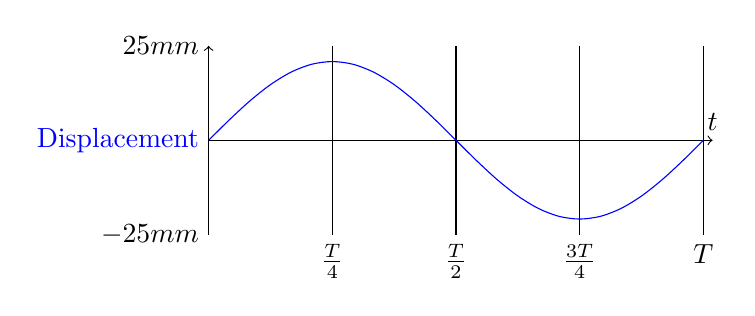
\begin{tikzpicture}[domain=0:6.282, smooth,variable=\x]
     \draw[->] (0,0) -- (6.4,0) node[above] {$t$};
  \draw[->] (0,-1.2)node[left] {$-25\text{mm}$} -- (0,1.2)node[left] {$25\text{mm}$};
  \draw (1.571,-1.2) node[below] {$\frac{T}{4}$} -- (1.571,1.2);
   \draw (3.141,-1.2) node[below] {$\frac{T}{2}$} -- (3.141,1.2);
    \draw (4.712,-1.2) node[below] {$\frac{3T}{4}$} -- (4.712,1.2);
     \draw (6.282,-1.2) node[below] {$T$} -- (6.282,1.2);
 \draw[color=blue] node[left] {Displacement}  plot (\x,{sin(\x r)}) ;
    \end{tikzpicture}
  %  }{Displacement of an oscillating object with parts of its cycle marked. }
    \caption{Displacement of an oscillating object with parts of its cycle marked. }
        \label{fig: shm with parts}
\end{figure}

a) When $t=\frac{1}{4}T$ the object is at the maximum amplitude $25\text{mm}$ away from equilibrium and is turning around to head back towards equilibrium.\\

b) When $t=\frac{1}{2}T$ the object passing through equilibrium, $x=0\text{mm}$, and heading away from equilibrium towards a negative displacement. \\

c) When $t=\frac{3}{4}T$ the object is at the maximum negative extension, $x=-25\text{mm}$, and is turning around to head back to equilibrium.\\

d) When $t=T$ the object is again passing through equilibrium, $x=0\text{mm}$, and moving away from it towards positive displacements.\\

You may have recognised already that shm is really uniform circular motion in disguise. \cref{fig: shm circle} shows a point $p$ rotating round on a circle. The coordinates of the point $p$ are found, using trigonometry on the triangle with hypotenuse $r$, to be
\begin{equation*}
x=r\cos\uptheta, \qquad y=r\sin\uptheta.
\end{equation*}
Also note that since $p$ is undergoing uniform circular motion its acceleration is given by\footnote{The minus sign is just showing that $a$ points towards the centre of the circle. We did not explicitly included it in the last section as there we only cared about the magnitude of the acceleration and were saying in words that this pointed towards the centre of the circle.} $a=-v^{2}/r$, where $v$ is the linear speed and $r$ is the radius of the circle. We also know that $v=\upomega r$ which implies that
\begin{equation*}
a=-\upomega^{2}r,
\end{equation*}
which is exactly what we expect for simple harmonic motion.

\begin{figure}[ht]
    \centering
    \ThisAltText{ A plot of a circle showing the decomposition of the radius into horizontal and vertical components. Both of these components will look like they are oscillating if we study them independently.}
  %  \pdftooltip{
    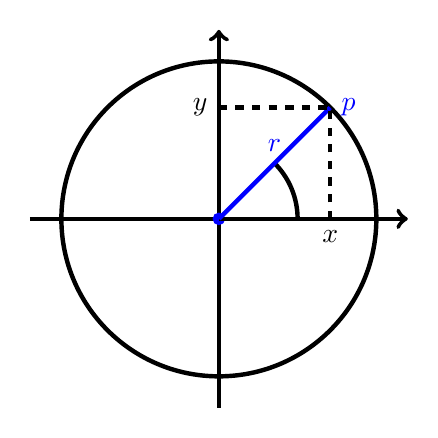
\begin{tikzpicture}
   % \draw[step=1cm,gray,very thin] (3,-3) grid (3,3);
   \draw[->,ultra thick] (0,-2.4)--(0,2.4);
     \draw[->,ultra thick] (-2.4,0)--(2.4,0);
   \filldraw[color = blue, ultra thick](0,0) circle (0.05);
    \draw[ ultra thick](0,0) circle (2);
    \draw[ultra thick] (0,0) -- (2,0);
    \draw[ultra thick] (1,0) arc (0:45:1) node[anchor=north]{$\uptheta$};
     %\draw[ultra thick, color=red] (2,0) arc (0:45:2) node[anchor=north]{$s$};
     \draw[color = blue, ultra thick](0,0)--node[above]{$r$}(1.414,1.414) node[right]{$p$} ;
     \draw[dashed, ultra thick] (0,1.414)node[left]{$y$} --(1.414,1.414);
      \draw[dashed, ultra thick] (1.414,0) node[below]{$x$}--(1.414,1.414);
    \end{tikzpicture}
   % }{Converting from SHM to circular motion}
    \caption{Converting from shm to circular motion.}
        \label{fig: shm circle}
\end{figure}

We can make another direct link between circular motion and shm. If we projected the circular motion onto the $y$-axis then it says that as time goes on the $y$ coordinate of $p$ increases to a maximum then decreases to $0$, keeps decreasing to a minimum, and then increases back to $0$ again. This is just the motion of a vertical spring oscillating around equilibrium. The $y$ component of the acceleration is $a_{y}=a\sin\uptheta$ and since $y=r\sin\uptheta$ we have that
\begin{equation*}
a_{y}=-\upomega^{2} r\sin\uptheta=-\upomega^{2}y.
\end{equation*}
This is the definition of shm.\\

What the relationship between shm and circular motion tells us is that the displacement (as well as the velocity and acceleration) of our oscillating object is described by trigonometric functions:
\begin{equation}
x=A\sin\left(\upomega t+\upphi\right).
\end{equation}
Here $A$ is the amplitude, $\upomega$ is the angular frequency, and $\upphi$ is a phase difference\footnote{You may be wondering why there is a phase difference here. It is because we can think about starting to observe the motion at any point, and we want to be able to relate this to starting from $x=0$ at $t=0$, this is what $\upphi$ takes in to account.}. For our example of motion on a circle up above we have that $A=r$ so the amplitude is the radius of the circle.\\

\textbf{Warning!} Remember that we need to measure $\uptheta=\upomega t$ in radians rather than degrees. we will also sometimes say frequency we will mean $\upomega$ rather than $f$, in practice it is best to compute both of them if asked to find the frequency.\\

\paragraph{Example 7.3:} An object oscillates with a time period of $T=3\text{s}$ and an amplitude of $A=58\text{mm}$. Calculate:
\begin{itemize}
\setlength{\itemsep}{-5pt}
    \item[a)] The frequency of oscillation,
    \item[b)] The maximum acceleration.
\end{itemize}  

a) The frequency is given by $f=1/T=1/3=0.33\text{Hz}$ and the angular frequency is $\upomega=2\uppi f=2.1\text{rads}^{-1}$.\\

b) The acceleration is maximum when the displacement has its maximum negative value, see the graphs in \cref{fig: shm profile} to check that this is true. This means that
\begin{equation*}
a_{\text{max}}=-\upomega^{2}(-A)=-(2.1)^{2}\times (-58\times10^{-3})=0.26\text{m/s}^{2}.
\end{equation*}

We call the shape of the curves in \cref{fig: shm profile} \textbf{sinusoidal}. You may have heard that name before, and you should see more about sinusoidal curves in the applied maths module.


\section{Springs and Pendulums}
\paragraph{Springs:} For an oscillating object the resultant force causing the acceleration is a restoring force acting towards the equilibrium position. As long as $F\propto -x$ we have that $a\propto -x$ and the motion is simple harmonic motion. For a spring the constant of proportionality between the restoring force and the displacement, in this case called the \textbf{extension}, is the spring constant $k$. The restoring force for a spring,  
\begin{equation}
F=-k x,
\label{eq: Hookes law}
\end{equation}
is given by Hooke's law. The spring constant essentially measures how stiff the spring is, or how hard it is to stretch the spring.  In our discussion about energy we saw a very similar expression but without the negative sign, that was because in \cref{sec: work and energy} when we quoted $F$ we meant the force needed to stretch the spring points away from equilibrium. While in \cref{eq: Hookes law}, $F$ is the restoring force pointing towards the springs equilibrium. Sometimes the restoring force will be denoted $F_{r}$ to try and avoid confusion. However, it is often left to the reader to work out which sign should be used from the choice of force.\\

If we combine \cref{eq: Hookes law} with both Newton's second law ($F=ma$) we see that
\begin{equation*}
a=-\frac{k}{m}x.
\end{equation*}
comparing this with the expression for acceleration in shm ($a=-\upomega^{2}x$) we get 
\begin{equation}
\upomega^{2}=\frac{k}{m}.
\end{equation}

So for any spring, in a regime where we can assume it undergoes shm, the angular frequency is determined entirely by the spring constant and the mass on the end of the spring. This means that we could set up a mass and spring system on a different planet and it would oscillate at the same rate. This will not be the case when we look at pendulums. Pendulums care what planet they are on but springs do not.\\

Notice that I have said this is only true if we are in a regime where we can assume a spring is a \textbf{simple harmonic oscillator}, ie an object undergoing simple harmonic motion. If we put too much mass on the end of a spring we can over stretch it and cause it to deform which means that it will no longer stretch and compress as it oscillates around equilibrium. You will some times see this expressed as Hooke's law only describing a spring in what is known as the (linear) \textbf{elastic regime}, ie where deformations are reversible. Going beyond this elastic regime means that the deformation is no longer reversible and the spring will be permanently deformed. Those of you going on to do Mechanical Engineering or Physics will learn more about this in the Materials module in your first year.\\

Recall that the period of oscillation is related to the angular frequency through $T=1/f=2\uppi/\upomega$. This means that the oscillation period of a spring is
\begin{equation}
T=\frac{2\uppi}{\upomega}=2\uppi\sqrt{\frac{m}{k}}.
\label{eq: spring period}
\end{equation}

If we have a vertical spring with a mass on the end then the spring will stretch until the restoring force of the spring $F_{r}$ balances the weight of the mass $F_{W}=mg$, ie the spring will extend until it reaches an equilibrium point where $F_{r}=F_{W}$. It is important to remember that the $x$ in Hooke's law is the extension of the spring \textbf{not} the length of the spring. The extension is the difference between the length of the spring with a mass attached, $L$, and the length of the spring with no mass attached, $L_{0}$. Or as an equation $x=L-L_{0}$. This distinction is important when you carry out the Hooke's law experiment in the lab sessions. Hooke's law says that the force needed to stretch the spring is proportional to the extension so if you plot $mg$ against $x$ you will find a linear relationship as we saw in \cref{fig: spring extension}. However, if you plot $mg$ against length then you will see a different relationship.

\paragraph{Example 7.4:} A spring of length $300\text{mm}$ hangs vertically with its upper end attached to a fixed point. When a small object of mass $0.2\text{kg}$ is suspended from the lower end of the spring in equilibrium, the spring is stretched to a length of $379\text{mm}$. Calculate:
\begin{itemize}
\setlength{\itemsep}{-5pt}
    \item[a)] The extension of the spring at equilibrium,
    \item[b)] The spring constant,
    \item[c)] The time period of oscillations if the mass were to be displaced slightly downward and released.
\end{itemize}  

a) The extension is the difference between the length with the mass, $L$, attached and the length without the mass attached, $L_{0}$. Above we denoted it by $x$ but we can make this clearer by calling the extension $\Delta L$ and calculating it from
\begin{equation*}
\Delta L=L-L_{0}=379-300=79\text{mm}.
\end{equation*}

b) The spring constant is calculated at equilibrium by comparing $F_{W}=mg$ and $F_{r}=-k\Delta L$
\begin{equation*}
-k\Delta L=mg , \quad \Rightarrow \, k=-\frac{mg}{\Delta L}=-\frac{0.2\times (-9.8)}{0.079}=25\text{N/m}.
\end{equation*}

c) For the period use
\begin{equation*}
T=2\uppi\sqrt{\frac{m}{k}}=2\uppi\sqrt{\frac{0.2}{25}}=0.56\text{s}.
\end{equation*}


\begin{figure}[ht]
    \centering
    \ThisAltText{ A picture of a simple pendulum taken from Wikimedia commons.}
   % \pdftooltip{
   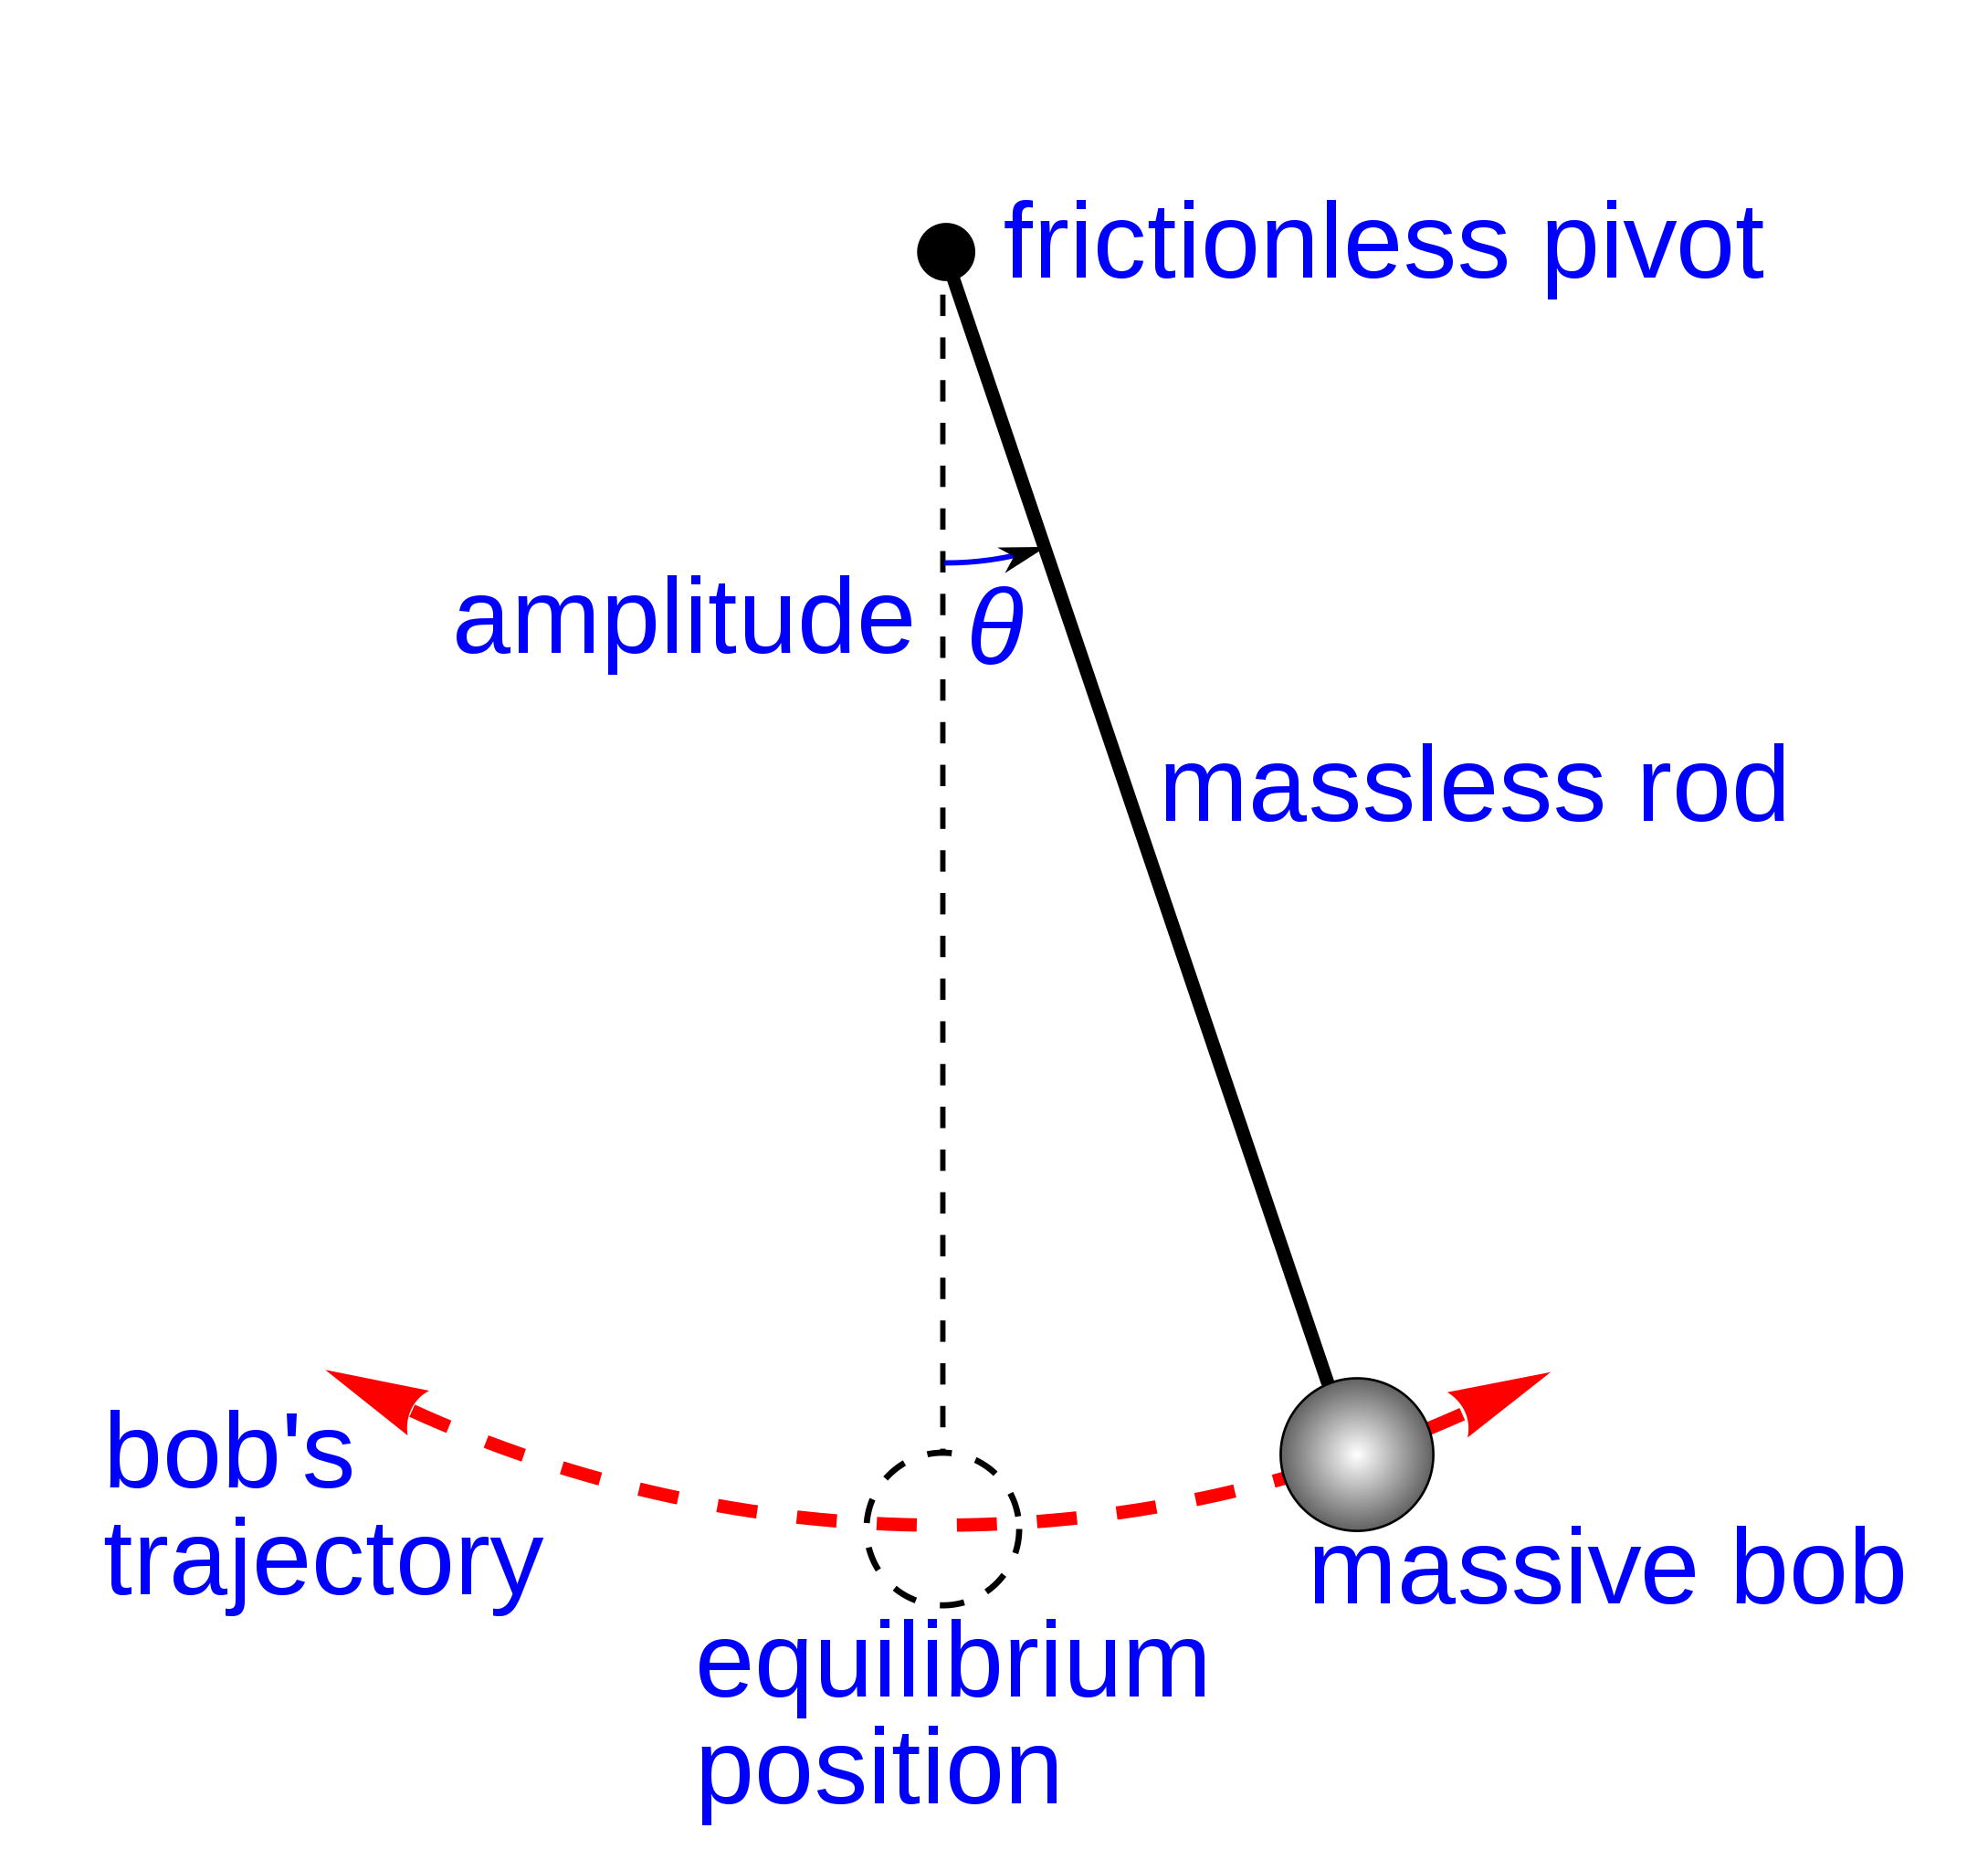
\includegraphics[width=0.6\textwidth]{figures/Simple_gravity_pendulum.png}
   %}{A schematic of the simple pendulum}
    \caption{A schematic of the simple pendulum from \href{https://commons.wikimedia.org/wiki/File:Simple_gravity_pendulum.svg}{Wikimedia Commons}.}
    \label{fig: simple pendulum}
\end{figure}


\paragraph{The simple pendulum:}  The other common example of simple harmonic motion is the \textbf{simple pendulum}. The basic set up is shown in \cref{fig: simple pendulum} and consists of a bob of mass $m$ on the end of a massless rod, or piece of string, of length $l$, we will also be making the assumption that the angular displacement $\uptheta$ is small\footnote{As the initial angle $\uptheta$ determines the amplitude we sometimes refer to $\uptheta$ itself as the amplitude. }. This is called a simple pendulum as it is a first approximation to the motion of a pendulum, it can be made more sophisticated by dropping the assumption that the the rod is massless and by considering initial displacements where the angle $\uptheta$ is large. We will not be very specific about what ``large'' means for $\uptheta$. However, in the lab sessions you will want to keep $\uptheta$ less than $20^{\circ}$ to be in this regime. Note that while I have given $\uptheta$ in degrees here we will need to work in radians for most of the mathematical expressions given in this section to be valid.\\

Equilibrium for this system is when the string hangs vertically downwards and with the tension in the string balancing the weight of the mass. If we displace the mass from equilibrium it will oscillate around its lowest point. In this case the restoring force is given by the horizontal component of the weight. The horizontal and vertical components are:
\begin{align*}
F_{\text{perp}}&=mg\cos\uptheta,\\
F_{\text{par}}&=-mg\sin\uptheta.
\end{align*}

\begin{figure}[ht]
    \centering
    \ThisAltText{ A triangle showing how the weight of the pendulum bob is decomposed into components.}
   % \pdftooltip{
   \begin{tikzpicture}[scale=2]
  \coordinate [label=left:$\theta$] (C) at (-1.5cm,-1.cm);
  \coordinate (A) at (1.5cm,-1.0cm);
  \coordinate (B) at (1.5cm,1.0cm);
  \draw (C) -- node[left] {$F_{W}=mg$} (B) -- node[right] {$mg\cos\uptheta$} (A) -- node[below] {$mg\sin\uptheta$} (C);
  \draw (1.25cm,-1.0cm) rectangle (1.5cm,-0.75cm);
  \tkzMarkAngle[size=1cm,color=blue](A,C,B)
 % \tkzMarkAngle[size=1cm,color=blue](C,B,A)
\end{tikzpicture}
%}{Components of the weight}
    \caption{The weight of the pendulum bob and its components. \textcolor{red}{This figure needs improved.}}
    \label{fig: weight components}
\end{figure}

The restoring force is thus $-mg\sin\uptheta$, while the tension in the rod balances the perpendicular component $F_{\text{perp}}$.  The restoring force leads to an acceleration through Newton's second law,
\begin{equation*}
a=\frac{F}{m}=-\frac{mg\sin\uptheta}{m}=-g\sin\uptheta.
\end{equation*}
When the angle is small we can use the approximation $\sin\uptheta\sim\uptheta=\frac{s}{l}$, where $s$ is the arc length. This means that
\begin{equation*}
a=-\frac{g}{l}s,
\end{equation*}
which is shm with an angular frequency of 
\begin{equation}
\upomega^{2}=\frac{g}{l},
\label{eq: pendulum frequency}
\end{equation}
and the period of oscillation is
\begin{equation}
T=\frac{2\uppi}{\upomega}=2\uppi\sqrt{\frac{l}{g}}.
\label{eq: pendulum period}
\end{equation}
Notice that unlike with a spring gravity is important.\\

As an aside note that we can think of the simple pendulum as being a ``spring'' with a mass dependent spring constant, $k_{\text{eff}}=\frac{mg}{l}$. This is related to an approximation scheme that is very common in physics where we use a a simple harmonic oscillator as a model for the low energy behaviour of many different phenomena.\\

Another point to be aware of is that the approximation that we used above, $\sin\uptheta\sim\uptheta$, is just the first term in what is known as a Taylor expansion where we can expand the $\sin$ function as
\begin{equation*}
\sin\uptheta=\uptheta-\frac{\uptheta^{3}}{3!}+\frac{\uptheta^{5}}{5!}-\dots, \qquad \text{for all } \uptheta.
\end{equation*}
If we want to understand the physics of a pendulum for angles larger than $10^{\circ}$ to $20^{\circ}$ more terms need to be included. This approximation is valid in both degrees and radians, however, if we then go on and use that $\uptheta=\frac{s}{l}$ in terms of the arc length, this is only valid if $\uptheta$ is measured in radians.\\

The expression for the period of the pendulum in \cref{eq: pendulum period} shows that the period can be changed by lengthening the string of pendulum rod. As mentioned above, the period would also change if the pendulum was set up on a planet with different gravity.\\

We can analyse oscillations by considering how the types of energy change during the motion. In particular, for a pendulum at its maximum displacement the bob is instantaneously at rest, since the motion is changing direction, and all of the energy is potential. While when the pendulum bob is passing through equilibrium all of the energy is kinetic.\\

In general the potential energy of a spring is
\begin{equation*}
E_{P}=\frac{1}{2}kx^{2},
\end{equation*} 
where $x$ is the displacement from equilibrium. Since at the maximum amplitude, $x=A$ all of the energy is potential, the total energy is
\begin{equation*}
E=\frac{1}{2}kA^{2}.
\end{equation*}
Since the total energy is $E_{K}+E_{P}$ the kinetic energy of the spring can be expressed as
\begin{equation*}
E_{K}=\frac{1}{2}\left(A^{2}-x^{2}\right).
\end{equation*}

We can use this to find a linear speed\footnote{As in this is the speed that the object has is we think of it as a moving in one dimension.} for the object at a displacement of $x$ from equilibrium. To do this write $E_{K}=\frac{1}{2}mv^{2}$ and equate the two expressions for the kinetic energy:
\begin{align*}
\frac{1}{2}mv^{2}&=\frac{1}{2}k\left(A^{2}-x^{2}\right),\\
\Rightarrow \, v^{2}&=\frac{k}{m}\left(A^{2}-x^{2}\right)=\upomega^{2}\left(A^{2}-x^{2}\right),
\end{align*}
which means that
\begin{equation*}
v=\pm\upomega\sqrt{A^{2}-x^{2}}.
\end{equation*}
Note that this fits our intuition that the velocity should be maximum at equilibrium where $x=0$, and zero at the maximum displacement, $x=\pm A$. If we plot both $E_{K}$ and $E_{P}$ we see that they are both parabolas, and the total energy is just a straight line. \textcolor{red}{This figure needs to be added.}

\section{Damping, Forcing, and Resonance}
So far we have studied oscillating objects while ignoring friction, air resistance, and any other force which may cause the oscillations to gradually die away. These are known as dissipative forces, and are essential when trying to match up our idealised models of oscillators with how real oscillators behave. We call the motion \textbf{damped} if there are dissipative forces. If we ant to make our models realistic we have to consider these dissipative effects along with phenomena like forcing and resonance. This section of the module is much more qualitative than the others. It can be made quantitative but the full mathematical description is more advanced than we want to be concerned with in this module. If you go on to study more physics during your degree then you will likely get to learn more about the maths behind these phenomena. If you want to know more now, then you can ask in the lectures or take a look at the further reading suggestions. \\

There are three types of damping that we are interested in here.
\begin{itemize}
\setlength{\itemsep}{-5pt}
    \item \textbf{Light damping:} This is when the time period is independent of the amplitude so each cycle of oscillation takes the same time, but the amplitude is gradually decreasing as the oscillations die away. 
    \item \textbf{Critical damping:} There is just enough damping to stop the system from oscillating after it has been displaced. This type of damping returns the oscillating object to equilibrium by the shortest possible route.
    \item \textbf{Heavy damping:} This occurs when the damping is so strong that no oscillating motion occurs and the mass returns to equilibrium straight away, but by a much slower route than for critical damping.
\end{itemize}  

\paragraph{Example 7.5:} Consider the following cases of damping and decide if they are light, critical, or heavy:
\begin{itemize}
\setlength{\itemsep}{-5pt}
    \item[a)] A child on a swing displaced from equilibrium and then released,
    \item[b)] A car suspension system,
    \item[c)] The door closer on a fire door.
\end{itemize}  

a) This is lightly damped as the swing will keep oscillating with the amplitude gradually decreasing as it returns to equilibrium. \\

b) Suspension is critically damped as we want the car to return to equilibrium as quickly as possible to avoid throwing the passengers around.\\

c) This is heavily damped as there are no oscillations, the closer ensures that the door returns to equilibrium, closed, in a slow and gentle manner.\\


As well as considering dissipative forces that damp an oscillator we can imagine adding forces that drive the oscillator. Imagine pushing someone on a swing, we are applying an external force, the push, to drive the motion of the oscillator rather than just displacing them from equilibrium and leaving them to oscillate back and forth. If we time our pushes well then they make the sing go higher and higher. This is known as \textbf{driving} or \textbf{forcing} the oscillation since we are applying an external force. These pushes are a periodic force, eg a force applied at regular intervals. When there is no external periodic force being applied we say that an oscillating system is oscillating at its \textbf{natural frequency}. When a periodic force is applied, we call it a \textbf{forced vibration}. In this case the response, ie the oscillation frequency, depends on the frequency of the forcing.\\

Consider forcing a spring, we could do this by just stretching and compressing the spring by hand, the frequency of oscillation is the applied frequency. A natural question is ``what happens if the applied frequency is increased?'' 

As the applied frequency increases from zero we would notice a few things happening. First, the amplitude of oscillation will initially increase, until it reaches some maximum amplitude at a particular applied frequency before starting to decrease as the frequency continues to be raised. The phase difference between the displacement of the oscillating object and the applied force increases from $0$ to $\uppi/2$, reaching $\uppi$ when the amplitude reaches its maximum value. The phase difference will then keep increasing up to $\uppi$ as the applied frequency is increased further. It would then keep increasing up to a phase difference of $2\uppi$ which is equivalent to a difference of $0$.\\

When the system is oscillating with its maximum amplitude, the phase difference between the driving force and the displacement is $\uppi/2$. This means that the driving force is in phase with the oscillators velocity and we say that the system is in \textbf{resonance}. The frequency at the maximum amplitude is called the \textbf{resonant frequency}. The lighter the damping the larger the maximum amplitude is at resonance and the closer that the resonant frequency is to the natural frequency. If there is no damping then the maximum amplitude would diverge at resonance, in practice this means that systems break when they reach resonance. On the other hand, if the damping is large enough then resonance can essentially be removed entirely. A famous example is the collapse of the Tacoma bridge. With a bridge like this we model it on an oscillator since it can be springy and bounce when someone walks across it. Most bridges are fitted with dampers so that resonance is avoided, this is very important since the steps of people walking across the bridge act like a periodic driving force.
